%%%%%%%%%%%%%%%%%%%%%%%%%%%%%%%%%%%%%%%%%%%%%%%%%%%%%%%%%%%%%%%%%%%%%%%%%%%%%%%%%%%%%%%%%
%
% v0p25 (May 15) - 3rd round of comments from referee
%
% v0p24 (May 1) - further reduction in text and some corrections - Xin
%
% v0p23 (April 30) - text editing to reduce the total length - Xin
%
% v0p22 (April 19) - Respond to the 2nd round of referees' comments
%
% v0p21 (Feb. 25) - Respond to referee's comments
%
% --- Xin Dong - further shortened to meet the length limit
%
% v0p17 (Dec. 19) - Collaboration review comments from Yale.
%
% v0p16 (Dec. 15) - Collaboration review comments from NISER.
%
% v0p15 (Dec. 12) - Collaboration review comments from Bill, CTU, Indiana.U, Tsinghua.U
%
% v0p14 (Nov. 25) - Further iteration from v13
%
% v0p13 (Nov. 13) - Further iteration from v12
%
% v0p12 (Nov. 13) - Comments from All GPC members
%
% v0p11 (Nov. 8) - improvements discussion about IMR
%
% v0p10 (Nov. 4) - Further reduction
%
% v0p9 (Nov. 2) - Comments from Huan
%
% v0p8 (Oct. 29) - Updated the text related to figure 3.
%
% v0p7 (...) -
%
% v0p6 (July 1) - Comments from Lijuan and Xianglei received
%
% v0p5 (June 11) - Comments Frank on the second part of the paper, synchronize the mass regions in the text
%
% v0p4 (June 6) - Fixed figure captions, Comments from Frank till line 275
%
% v0p3 (May 30) - Final figures from Jie
%
% v0p2 (May 29) - Comments from Joey on wording (March 29)
%
% v0p1 (Mar. 26) - Some wording improvements
%
% v0p0 (Jan. 17) - first PRL version (reference sorted, spelling checked)
%                            - Jan 19, fig updated
%
%%%%%%%%%%%%%%%%%%%%%%%%%%%%%%%%%%%%%%%%%%%%%%%%%%%%%%%%%%%%%%%%%%%%%%%%%%%%%%%%%%%%%%%%%%
% ****** Start of file apssamp.tex ******
%
%   This file is part of the APS files in the REVTeX 4 distribution.
%   Version 4.0 of REVTeX, August 2001
%
%   Copyright (c) 2001 The American Physical Society.
%
%   See the REVTeX 4 README file for restrictions and more information.
%
% TeX'ing this file requires that you have AMS-LaTeX 2.0 installed
% as well as the rest of the prerequisites for REVTeX 4.0
%
% See the REVTeX 4 README file
% It also requires running BibTeX. The commands are as follows:
%
%  1)  latex apssamp.tex
%  2)  bibtex apssamp
%  3)  latex apssamp.tex
%  4)  latex apssamp.tex
%
%\RequirePackage{lineno}
%\RequirePackage[mathlines]{lineno}
%\RequirePackage[pagewise,mathlines]{lineno}
%\documentclass[twocolumn,showpacs,amsmath,amssymb,linenumbers,superscriptaddress,nofootinbib]{revtex4-1}
\documentclass[twocolumn,showpacs,amsmath,amssymb,superscriptaddress,nofootinbib]{revtex4-1}
%\documentclass[10pt,aps,prc,twocolumn,floatfix,showpacs,superscriptaddress]{revtex4-1}
%\documentclass[twocolumn,showpacs,amsmath,amssymb,linenumbers]{revtex4-1}
%\documentclass[twocolumn,showpacs,preprintnumbers,amsmath,amssymb,linenumbers]{revtex4-1}
%\documentclass[preprint,showpacs,preprintnumbers,amsmath,amssymb]{revtex4}

% Some other (several out of many) possibilities
%\documentclass[preprint,aps]{revtex4}
%\documentclass[preprint,aps,draft]{revtex4}
%\documentclass[prb]{revtex4}% Physical Review B
%\documentclass[12pt]{article}

\textheight 9.0in \textwidth 6.5in \oddsidemargin 10pt
\evensidemargin 0pt \topmargin 0pt

\usepackage{graphicx}% Include figure files
\usepackage{dcolumn}% Align table columns on decimal point
\usepackage{bm}% bold math
\usepackage{color}
%\usepackage{lineno}
\usepackage{ulem}
\usepackage{url}
\usepackage{multirow}

\newcommand{\bfg }{\begin{figure}[htpb]}
\newcommand{\efg }{\end{figure}}
\newcommand{\bmn }{\begin{minipage}}
\newcommand{\emn }{\end{minipage}}
\newcommand{\bt }{\begin{table}[htpb]}
\newcommand{\et }{\end{table}}
\newcommand{\pp }{$p$ + $p$ }
\newcommand{\dAu}{\textit{d}+Au }
\newcommand{\srt}{$\sqrt{s}$ }
\newcommand{\sNN}{$\sqrt{s_{\rm NN}}$ }
\newcommand{\mpt}{$\langle p_T \rangle$ }
\newcommand{\met}{$\langle E_T \rangle$ }
\newcommand{\pt}{$p_T$ }
\newcommand{\etal}{{\it et al.}}
\newcommand{\GeVc}{GeV/$c$ }
\newcommand{\GeVcsq}{GeV/$c^2$ }
\newcommand{\Dzero}{$D^{0}$ }
\newcommand{\Dzerobar}{$\overline{D^{0}}$ }
\newcommand{\Dstar}{$D^{*}$ }
\newcommand{\Dstarpm}{$D^{*\pm}$}
\newcommand{\dsigmady}{$d\sigma/dy|_{y=0}^{c\bar{c}}$}

\newcommand{ \be }{\begin{equation}}
\newcommand{ \ee }{\end{equation}}
\newcommand{ \bea }{\begin{eqnarray}}
\newcommand{ \eea }{\end{eqnarray}}
\newcommand{ \la }{\langle}
\newcommand{ \ra }{\rangle}
\newcommand{ \eps }{{\varepsilon}}
\newcommand{ \rar }{\rightarrow}
\newcommand{ \lar }{\leftarrow}
\newcommand{ \as }{$\alpha_{\rm s}$ }
\newcommand{ \pT }{$p_{\rm T}$ }
\newcommand{ \Ncoll}{$N_{\rm coll}$}
\newcommand{ \Npart}{$N_{\rm part}$}

%--===================================================================

\begin{document}
% A useful Journal macro
\def\Journal#1#2#3#4{{#1} {\bf #2}, #3 (#4)}

% Some useful journal names
\def\NCA{Nuovo Cimento}
\def\NIM{Nucl. Instr. Meth.}
\def\NIMA{{Nucl. Instr. Meth.} A}
\def\NPB{{Nucl. Phys.} B}
\def\NPA{{Nucl. Phys.} A}
\def\PLB{{Phys. Lett.}  B}
\def\PRL{{Phys. Rev. Lett.}}
\def\PRC{{Phys. Rev.} C}
\def\PRD{{Phys. Rev.} D}
\def\ZPC{{Z. Phys.} C}
\def\JPG{{J. Phys.} G}
\def\EPJ{{Eur. Phys. J.} C}
\def\EPJA{{Eur. Phys. J.} A}
\def\EPJST{{Eur. Phys. J.} - Special Topics}
\def\RPP{{Rep. Prog. Phys.}}
\def\PR{{Phys. Rep.}}
\def\ANP{{Adv. Nucl. Phys.}}

%\preprint{}

%{\it version 0.14}

\title{Dielectron Mass Spectra from Au+Au Collisions at \sNN = 200\,GeV}

%\collaboration{STAR
%Collaboration}\homepage{www.star.bnl.gov}\noaffiliation
\affiliation{AGH University of Science and Technology, Cracow, Poland}
\affiliation{Argonne National Laboratory, Argonne, Illinois 60439, USA}
\affiliation{University of Birmingham, Birmingham, United Kingdom}
\affiliation{Brookhaven National Laboratory, Upton, New York 11973, USA}
\affiliation{University of California, Berkeley, California 94720, USA}
\affiliation{University of California, Davis, California 95616, USA}
\affiliation{University of California, Los Angeles, California 90095, USA}
\affiliation{Universidade Estadual de Campinas, Sao Paulo, Brazil}
\affiliation{Central China Normal University (HZNU), Wuhan 430079, China}
\affiliation{University of Illinois at Chicago, Chicago, Illinois 60607, USA}
\affiliation{Cracow University of Technology, Cracow, Poland}
\affiliation{Creighton University, Omaha, Nebraska 68178, USA}
\affiliation{Czech Technical University in Prague, FNSPE, Prague, 115 19, Czech Republic}
\affiliation{Nuclear Physics Institute AS CR, 250 68 \v{R}e\v{z}/Prague, Czech Republic}
\affiliation{Frankfurt Institute for Advanced Studies FIAS, Germany}
\affiliation{Institute of Physics, Bhubaneswar 751005, India}
\affiliation{Indian Institute of Technology, Mumbai, India}
\affiliation{Indiana University, Bloomington, Indiana 47408, USA}
\affiliation{Alikhanov Institute for Theoretical and Experimental Physics, Moscow, Russia}
\affiliation{University of Jammu, Jammu 180001, India}
\affiliation{Joint Institute for Nuclear Research, Dubna, 141 980, Russia}
\affiliation{Kent State University, Kent, Ohio 44242, USA}
\affiliation{University of Kentucky, Lexington, Kentucky, 40506-0055, USA}
\affiliation{Korea Institute of Science and Technology Information, Daejeon, Korea}
\affiliation{Institute of Modern Physics, Lanzhou, China}
\affiliation{Lawrence Berkeley National Laboratory, Berkeley, California 94720, USA}
\affiliation{Massachusetts Institute of Technology, Cambridge, MA 02139-4307, USA}
\affiliation{Max-Planck-Institut f\"ur Physik, Munich, Germany}
\affiliation{Michigan State University, East Lansing, Michigan 48824, USA}
\affiliation{Moscow Engineering Physics Institute, Moscow Russia}
\affiliation{National Institute of Science Education and Research, Bhubaneswar 751005, India}
\affiliation{Ohio State University, Columbus, Ohio 43210, USA}
\affiliation{Old Dominion University, Norfolk, VA, 23529, USA}
\affiliation{Institute of Nuclear Physics PAN, Cracow, Poland}
\affiliation{Panjab University, Chandigarh 160014, India}
\affiliation{Pennsylvania State University, University Park, Pennsylvania 16802, USA}
\affiliation{Institute of High Energy Physics, Protvino, Russia}
\affiliation{Purdue University, West Lafayette, Indiana 47907, USA}
\affiliation{Pusan National University, Pusan, Republic of Korea}
\affiliation{University of Rajasthan, Jaipur 302004, India}
\affiliation{Rice University, Houston, Texas 77251, USA}
\affiliation{Universidade de Sao Paulo, Sao Paulo, Brazil}
\affiliation{University of Science \& Technology of China, Hefei 230026, China}
\affiliation{Shandong University, Jinan, Shandong 250100, China}
\affiliation{Shanghai Institute of Applied Physics, Shanghai 201800, China}
\affiliation{SUBATECH, Nantes, France}
\affiliation{Temple University, Philadelphia, Pennsylvania, 19122, USA}
\affiliation{Texas A\&M University, College Station, Texas 77843, USA}
\affiliation{University of Texas, Austin, Texas 78712, USA}
\affiliation{University of Houston, Houston, TX, 77204, USA}
\affiliation{Tsinghua University, Beijing 100084, China}
\affiliation{United States Naval Academy, Annapolis, MD 21402, USA}
\affiliation{Valparaiso University, Valparaiso, Indiana 46383, USA}
\affiliation{Variable Energy Cyclotron Centre, Kolkata 700064, India}
\affiliation{Warsaw University of Technology, Warsaw, Poland}
\affiliation{University of Washington, Seattle, Washington 98195, USA}
\affiliation{Yale University, New Haven, Connecticut 06520, USA}
\affiliation{University of Zagreb, Zagreb, HR-10002, Croatia}

\author{L.~Adamczyk}\affiliation{AGH University of Science and Technology, Cracow, Poland}
\author{J.~K.~Adkins}\affiliation{University of Kentucky, Lexington, Kentucky, 40506-0055, USA}
\author{G.~Agakishiev}\affiliation{Joint Institute for Nuclear Research, Dubna, 141 980, Russia}
\author{M.~M.~Aggarwal}\affiliation{Panjab University, Chandigarh 160014, India}
\author{Z.~Ahammed}\affiliation{Variable Energy Cyclotron Centre, Kolkata 700064, India}
\author{I.~Alekseev}\affiliation{Alikhanov Institute for Theoretical and Experimental Physics, Moscow, Russia}
\author{J.~Alford}\affiliation{Kent State University, Kent, Ohio 44242, USA}
\author{C.~D.~Anson}\affiliation{Ohio State University, Columbus, Ohio 43210, USA}
\author{A.~Aparin}\affiliation{Joint Institute for Nuclear Research, Dubna, 141 980, Russia}
\author{D.~Arkhipkin}\affiliation{Brookhaven National Laboratory, Upton, New York 11973, USA}
\author{E.~C.~Aschenauer}\affiliation{Brookhaven National Laboratory, Upton, New York 11973, USA}
\author{G.~S.~Averichev}\affiliation{Joint Institute for Nuclear Research, Dubna, 141 980, Russia}
\author{A.~Banerjee}\affiliation{Variable Energy Cyclotron Centre, Kolkata 700064, India}
\author{Z.~Barnovska~}\affiliation{Nuclear Physics Institute AS CR, 250 68 \v{R}e\v{z}/Prague, Czech Republic}
\author{D.~R.~Beavis}\affiliation{Brookhaven National Laboratory, Upton, New York 11973, USA}
\author{R.~Bellwied}\affiliation{University of Houston, Houston, TX, 77204, USA}
\author{A.~Bhasin}\affiliation{University of Jammu, Jammu 180001, India}
\author{A.~K.~Bhati}\affiliation{Panjab University, Chandigarh 160014, India}
\author{P.~Bhattarai}\affiliation{University of Texas, Austin, Texas 78712, USA}
\author{H.~Bichsel}\affiliation{University of Washington, Seattle, Washington 98195, USA}
\author{J.~Bielcik}\affiliation{Czech Technical University in Prague, FNSPE, Prague, 115 19, Czech Republic}
\author{J.~Bielcikova}\affiliation{Nuclear Physics Institute AS CR, 250 68 \v{R}e\v{z}/Prague, Czech Republic}
\author{L.~C.~Bland}\affiliation{Brookhaven National Laboratory, Upton, New York 11973, USA}
\author{I.~G.~Bordyuzhin}\affiliation{Alikhanov Institute for Theoretical and Experimental Physics, Moscow, Russia}
\author{W.~Borowski}\affiliation{SUBATECH, Nantes, France}
\author{J.~Bouchet}\affiliation{Kent State University, Kent, Ohio 44242, USA}
\author{A.~V.~Brandin}\affiliation{Moscow Engineering Physics Institute, Moscow Russia}
\author{S.~G.~Brovko}\affiliation{University of California, Davis, California 95616, USA}
\author{S.~B{\"u}ltmann}\affiliation{Old Dominion University, Norfolk, VA, 23529, USA}
\author{I.~Bunzarov}\affiliation{Joint Institute for Nuclear Research, Dubna, 141 980, Russia}
\author{T.~P.~Burton}\affiliation{Brookhaven National Laboratory, Upton, New York 11973, USA}
\author{J.~Butterworth}\affiliation{Rice University, Houston, Texas 77251, USA}
\author{H.~Caines}\affiliation{Yale University, New Haven, Connecticut 06520, USA}
\author{M.~Calder\'on~de~la~Barca~S\'anchez}\affiliation{University of California, Davis, California 95616, USA}
\author{D.~Cebra}\affiliation{University of California, Davis, California 95616, USA}
\author{R.~Cendejas}\affiliation{Pennsylvania State University, University Park, Pennsylvania 16802, USA}
\author{M.~C.~Cervantes}\affiliation{Texas A\&M University, College Station, Texas 77843, USA}
\author{P.~Chaloupka}\affiliation{Czech Technical University in Prague, FNSPE, Prague, 115 19, Czech Republic}
\author{Z.~Chang}\affiliation{Texas A\&M University, College Station, Texas 77843, USA}
\author{S.~Chattopadhyay}\affiliation{Variable Energy Cyclotron Centre, Kolkata 700064, India}
\author{H.~F.~Chen}\affiliation{University of Science \& Technology of China, Hefei 230026, China}
\author{J.~H.~Chen}\affiliation{Shanghai Institute of Applied Physics, Shanghai 201800, China}
\author{L.~Chen}\affiliation{Central China Normal University (HZNU), Wuhan 430079, China}
\author{J.~Cheng}\affiliation{Tsinghua University, Beijing 100084, China}
\author{M.~Cherney}\affiliation{Creighton University, Omaha, Nebraska 68178, USA}
\author{A.~Chikanian}\affiliation{Yale University, New Haven, Connecticut 06520, USA}
\author{W.~Christie}\affiliation{Brookhaven National Laboratory, Upton, New York 11973, USA}
\author{J.~Chwastowski}\affiliation{Cracow University of Technology, Cracow, Poland}
\author{M.~J.~M.~Codrington}\affiliation{University of Texas, Austin, Texas 78712, USA}
\author{J.~G.~Cramer}\affiliation{University of Washington, Seattle, Washington 98195, USA}
\author{H.~J.~Crawford}\affiliation{University of California, Berkeley, California 94720, USA}
\author{X.~Cui}\affiliation{University of Science \& Technology of China, Hefei 230026, China}
\author{S.~Das}\affiliation{Institute of Physics, Bhubaneswar 751005, India}
\author{A.~Davila~Leyva}\affiliation{University of Texas, Austin, Texas 78712, USA}
\author{L.~C.~De~Silva}\affiliation{University of Houston, Houston, TX, 77204, USA}
\author{R.~R.~Debbe}\affiliation{Brookhaven National Laboratory, Upton, New York 11973, USA}
\author{T.~G.~Dedovich}\affiliation{Joint Institute for Nuclear Research, Dubna, 141 980, Russia}
\author{J.~Deng}\affiliation{Shandong University, Jinan, Shandong 250100, China}
\author{A.~A.~Derevschikov}\affiliation{Institute of High Energy Physics, Protvino, Russia}
\author{R.~Derradi~de~Souza}\affiliation{Universidade Estadual de Campinas, Sao Paulo, Brazil}
\author{S.~Dhamija}\affiliation{Indiana University, Bloomington, Indiana 47408, USA}
\author{B.~di~Ruzza}\affiliation{Brookhaven National Laboratory, Upton, New York 11973, USA}
\author{L.~Didenko}\affiliation{Brookhaven National Laboratory, Upton, New York 11973, USA}
\author{C.~Dilks}\affiliation{Pennsylvania State University, University Park, Pennsylvania 16802, USA}
\author{F.~Ding}\affiliation{University of California, Davis, California 95616, USA}
\author{P.~Djawotho}\affiliation{Texas A\&M University, College Station, Texas 77843, USA}
\author{X.~Dong}\affiliation{Lawrence Berkeley National Laboratory, Berkeley, California 94720, USA}
\author{J.~L.~Drachenberg}\affiliation{Valparaiso University, Valparaiso, Indiana 46383, USA}
\author{J.~E.~Draper}\affiliation{University of California, Davis, California 95616, USA}
\author{C.~M.~Du}\affiliation{Institute of Modern Physics, Lanzhou, China}
\author{L.~E.~Dunkelberger}\affiliation{University of California, Los Angeles, California 90095, USA}
\author{J.~C.~Dunlop}\affiliation{Brookhaven National Laboratory, Upton, New York 11973, USA}
\author{L.~G.~Efimov}\affiliation{Joint Institute for Nuclear Research, Dubna, 141 980, Russia}
\author{J.~Engelage}\affiliation{University of California, Berkeley, California 94720, USA}
\author{K.~S.~Engle}\affiliation{United States Naval Academy, Annapolis, MD 21402, USA}
\author{G.~Eppley}\affiliation{Rice University, Houston, Texas 77251, USA}
\author{L.~Eun}\affiliation{Lawrence Berkeley National Laboratory, Berkeley, California 94720, USA}
\author{O.~Evdokimov}\affiliation{University of Illinois at Chicago, Chicago, Illinois 60607, USA}
\author{R.~Fatemi}\affiliation{University of Kentucky, Lexington, Kentucky, 40506-0055, USA}
\author{S.~Fazio}\affiliation{Brookhaven National Laboratory, Upton, New York 11973, USA}
\author{J.~Fedorisin}\affiliation{Joint Institute for Nuclear Research, Dubna, 141 980, Russia}
\author{P.~Filip}\affiliation{Joint Institute for Nuclear Research, Dubna, 141 980, Russia}
\author{E.~Finch}\affiliation{Yale University, New Haven, Connecticut 06520, USA}
\author{Y.~Fisyak}\affiliation{Brookhaven National Laboratory, Upton, New York 11973, USA}
\author{C.~E.~Flores}\affiliation{University of California, Davis, California 95616, USA}
\author{C.~A.~Gagliardi}\affiliation{Texas A\&M University, College Station, Texas 77843, USA}
\author{D.~R.~Gangadharan}\affiliation{Ohio State University, Columbus, Ohio 43210, USA}
\author{D.~ Garand}\affiliation{Purdue University, West Lafayette, Indiana 47907, USA}
\author{F.~Geurts}\affiliation{Rice University, Houston, Texas 77251, USA}
\author{A.~Gibson}\affiliation{Valparaiso University, Valparaiso, Indiana 46383, USA}
\author{M.~Girard}\affiliation{Warsaw University of Technology, Warsaw, Poland}
\author{S.~Gliske}\affiliation{Argonne National Laboratory, Argonne, Illinois 60439, USA}
\author{D.~Grosnick}\affiliation{Valparaiso University, Valparaiso, Indiana 46383, USA}
\author{Y.~Guo}\affiliation{University of Science \& Technology of China, Hefei 230026, China}
\author{A.~Gupta}\affiliation{University of Jammu, Jammu 180001, India}
\author{S.~Gupta}\affiliation{University of Jammu, Jammu 180001, India}
\author{W.~Guryn}\affiliation{Brookhaven National Laboratory, Upton, New York 11973, USA}
\author{B.~Haag}\affiliation{University of California, Davis, California 95616, USA}
\author{O.~Hajkova}\affiliation{Czech Technical University in Prague, FNSPE, Prague, 115 19, Czech Republic}
\author{A.~Hamed}\affiliation{Texas A\&M University, College Station, Texas 77843, USA}
\author{L.-X.~Han}\affiliation{Shanghai Institute of Applied Physics, Shanghai 201800, China}
\author{R.~Haque}\affiliation{National Institute of Science Education and Research, Bhubaneswar 751005, India}
\author{J.~W.~Harris}\affiliation{Yale University, New Haven, Connecticut 06520, USA}
\author{S.~Heppelmann}\affiliation{Pennsylvania State University, University Park, Pennsylvania 16802, USA}
\author{A.~Hirsch}\affiliation{Purdue University, West Lafayette, Indiana 47907, USA}
\author{G.~W.~Hoffmann}\affiliation{University of Texas, Austin, Texas 78712, USA}
\author{D.~J.~Hofman}\affiliation{University of Illinois at Chicago, Chicago, Illinois 60607, USA}
\author{S.~Horvat}\affiliation{Yale University, New Haven, Connecticut 06520, USA}
\author{B.~Huang}\affiliation{Brookhaven National Laboratory, Upton, New York 11973, USA}
\author{H.~Z.~Huang}\affiliation{University of California, Los Angeles, California 90095, USA}
\author{X.~ Huang}\affiliation{Tsinghua University, Beijing 100084, China}
\author{P.~Huck}\affiliation{Central China Normal University (HZNU), Wuhan 430079, China}
\author{T.~J.~Humanic}\affiliation{Ohio State University, Columbus, Ohio 43210, USA}
\author{G.~Igo}\affiliation{University of California, Los Angeles, California 90095, USA}
\author{W.~W.~Jacobs}\affiliation{Indiana University, Bloomington, Indiana 47408, USA}
\author{H.~Jang}\affiliation{Korea Institute of Science and Technology Information, Daejeon, Korea}
\author{E.~G.~Judd}\affiliation{University of California, Berkeley, California 94720, USA}
\author{S.~Kabana}\affiliation{SUBATECH, Nantes, France}
\author{D.~Kalinkin}\affiliation{Alikhanov Institute for Theoretical and Experimental Physics, Moscow, Russia}
\author{K.~Kang}\affiliation{Tsinghua University, Beijing 100084, China}
\author{K.~Kauder}\affiliation{University of Illinois at Chicago, Chicago, Illinois 60607, USA}
\author{H.~W.~Ke}\affiliation{Brookhaven National Laboratory, Upton, New York 11973, USA}
\author{D.~Keane}\affiliation{Kent State University, Kent, Ohio 44242, USA}
\author{A.~Kechechyan}\affiliation{Joint Institute for Nuclear Research, Dubna, 141 980, Russia}
\author{A.~Kesich}\affiliation{University of California, Davis, California 95616, USA}
\author{Z.~H.~Khan}\affiliation{University of Illinois at Chicago, Chicago, Illinois 60607, USA}
\author{D.~P.~Kikola}\affiliation{Warsaw University of Technology, Warsaw, Poland}
\author{I.~Kisel}\affiliation{Frankfurt Institute for Advanced Studies FIAS, Germany}
\author{A.~Kisiel}\affiliation{Warsaw University of Technology, Warsaw, Poland}
\author{D.~D.~Koetke}\affiliation{Valparaiso University, Valparaiso, Indiana 46383, USA}
\author{T.~Kollegger}\affiliation{Frankfurt Institute for Advanced Studies FIAS, Germany}
\author{J.~Konzer}\affiliation{Purdue University, West Lafayette, Indiana 47907, USA}
\author{I.~Koralt}\affiliation{Old Dominion University, Norfolk, VA, 23529, USA}
\author{W.~Korsch}\affiliation{University of Kentucky, Lexington, Kentucky, 40506-0055, USA}
\author{L.~Kotchenda}\affiliation{Moscow Engineering Physics Institute, Moscow Russia}
\author{P.~Kravtsov}\affiliation{Moscow Engineering Physics Institute, Moscow Russia}
\author{K.~Krueger}\affiliation{Argonne National Laboratory, Argonne, Illinois 60439, USA}
\author{I.~Kulakov}\affiliation{Frankfurt Institute for Advanced Studies FIAS, Germany}
\author{L.~Kumar}\affiliation{National Institute of Science Education and Research, Bhubaneswar 751005, India}
\author{R.~A.~Kycia}\affiliation{Cracow University of Technology, Cracow, Poland}
\author{M.~A.~C.~Lamont}\affiliation{Brookhaven National Laboratory, Upton, New York 11973, USA}
\author{J.~M.~Landgraf}\affiliation{Brookhaven National Laboratory, Upton, New York 11973, USA}
\author{K.~D.~ Landry}\affiliation{University of California, Los Angeles, California 90095, USA}
\author{J.~Lauret}\affiliation{Brookhaven National Laboratory, Upton, New York 11973, USA}
\author{A.~Lebedev}\affiliation{Brookhaven National Laboratory, Upton, New York 11973, USA}
\author{R.~Lednicky}\affiliation{Joint Institute for Nuclear Research, Dubna, 141 980, Russia}
\author{J.~H.~Lee}\affiliation{Brookhaven National Laboratory, Upton, New York 11973, USA}
\author{M.~J.~LeVine}\affiliation{Brookhaven National Laboratory, Upton, New York 11973, USA}
\author{C.~Li}\affiliation{University of Science \& Technology of China, Hefei 230026, China}
\author{W.~Li}\affiliation{Shanghai Institute of Applied Physics, Shanghai 201800, China}
\author{X.~Li}\affiliation{Purdue University, West Lafayette, Indiana 47907, USA}
\author{X.~Li}\affiliation{Temple University, Philadelphia, Pennsylvania, 19122, USA}
\author{Y.~Li}\affiliation{Tsinghua University, Beijing 100084, China}
\author{Z.~M.~Li}\affiliation{Central China Normal University (HZNU), Wuhan 430079, China}
\author{L.~M.~Lima}\affiliation{Universidade de Sao Paulo, Sao Paulo, Brazil}
\author{M.~A.~Lisa}\affiliation{Ohio State University, Columbus, Ohio 43210, USA}
\author{F.~Liu}\affiliation{Central China Normal University (HZNU), Wuhan 430079, China}
\author{T.~Ljubicic}\affiliation{Brookhaven National Laboratory, Upton, New York 11973, USA}
\author{W.~J.~Llope}\affiliation{Rice University, Houston, Texas 77251, USA}
\author{R.~S.~Longacre}\affiliation{Brookhaven National Laboratory, Upton, New York 11973, USA}
\author{X.~Luo}\affiliation{Central China Normal University (HZNU), Wuhan 430079, China}
\author{G.~L.~Ma}\affiliation{Shanghai Institute of Applied Physics, Shanghai 201800, China}
\author{Y.~G.~Ma}\affiliation{Shanghai Institute of Applied Physics, Shanghai 201800, China}
\author{D.~M.~M.~D.~Madagodagettige~Don}\affiliation{Creighton University, Omaha, Nebraska 68178, USA}
\author{D.~P.~Mahapatra}\affiliation{Institute of Physics, Bhubaneswar 751005, India}
\author{R.~Majka}\affiliation{Yale University, New Haven, Connecticut 06520, USA}
\author{S.~Margetis}\affiliation{Kent State University, Kent, Ohio 44242, USA}
\author{C.~Markert}\affiliation{University of Texas, Austin, Texas 78712, USA}
\author{H.~Masui}\affiliation{Lawrence Berkeley National Laboratory, Berkeley, California 94720, USA}
\author{H.~S.~Matis}\affiliation{Lawrence Berkeley National Laboratory, Berkeley, California 94720, USA}
\author{D.~McDonald}\affiliation{University of Houston, Houston, TX, 77204, USA}
\author{T.~S.~McShane}\affiliation{Creighton University, Omaha, Nebraska 68178, USA}
\author{N.~G.~Minaev}\affiliation{Institute of High Energy Physics, Protvino, Russia}
\author{S.~Mioduszewski}\affiliation{Texas A\&M University, College Station, Texas 77843, USA}
\author{B.~Mohanty}\affiliation{National Institute of Science Education and Research, Bhubaneswar 751005, India}
\author{M.~M.~Mondal}\affiliation{Texas A\&M University, College Station, Texas 77843, USA}
\author{D.~A.~Morozov}\affiliation{Institute of High Energy Physics, Protvino, Russia}
\author{M.~G.~Munhoz}\affiliation{Universidade de Sao Paulo, Sao Paulo, Brazil}
\author{M.~K.~Mustafa}\affiliation{Lawrence Berkeley National Laboratory, Berkeley, California 94720, USA}
\author{B.~K.~Nandi}\affiliation{Indian Institute of Technology, Mumbai, India}
\author{Md.~Nasim}\affiliation{National Institute of Science Education and Research, Bhubaneswar 751005, India}
\author{T.~K.~Nayak}\affiliation{Variable Energy Cyclotron Centre, Kolkata 700064, India}
\author{J.~M.~Nelson}\affiliation{University of Birmingham, Birmingham, United Kingdom}
\author{L.~V.~Nogach}\affiliation{Institute of High Energy Physics, Protvino, Russia}
\author{S.~Y.~Noh}\affiliation{Korea Institute of Science and Technology Information, Daejeon, Korea}
\author{J.~Novak}\affiliation{Michigan State University, East Lansing, Michigan 48824, USA}
\author{S.~B.~Nurushev}\affiliation{Institute of High Energy Physics, Protvino, Russia}
\author{G.~Odyniec}\affiliation{Lawrence Berkeley National Laboratory, Berkeley, California 94720, USA}
\author{A.~Ogawa}\affiliation{Brookhaven National Laboratory, Upton, New York 11973, USA}
\author{K.~Oh}\affiliation{Pusan National University, Pusan, Republic of Korea}
\author{A.~Ohlson}\affiliation{Yale University, New Haven, Connecticut 06520, USA}
\author{V.~Okorokov}\affiliation{Moscow Engineering Physics Institute, Moscow Russia}
\author{E.~W.~Oldag}\affiliation{University of Texas, Austin, Texas 78712, USA}
\author{R.~A.~N.~Oliveira}\affiliation{Universidade de Sao Paulo, Sao Paulo, Brazil}
\author{M.~Pachr}\affiliation{Czech Technical University in Prague, FNSPE, Prague, 115 19, Czech Republic}
\author{B.~S.~Page}\affiliation{Indiana University, Bloomington, Indiana 47408, USA}
\author{S.~K.~Pal}\affiliation{Variable Energy Cyclotron Centre, Kolkata 700064, India}
\author{Y.~X.~Pan}\affiliation{University of California, Los Angeles, California 90095, USA}
\author{Y.~Pandit}\affiliation{University of Illinois at Chicago, Chicago, Illinois 60607, USA}
\author{Y.~Panebratsev}\affiliation{Joint Institute for Nuclear Research, Dubna, 141 980, Russia}
\author{T.~Pawlak}\affiliation{Warsaw University of Technology, Warsaw, Poland}
\author{B.~Pawlik}\affiliation{Institute of Nuclear Physics PAN, Cracow, Poland}
\author{H.~Pei}\affiliation{Central China Normal University (HZNU), Wuhan 430079, China}
\author{C.~Perkins}\affiliation{University of California, Berkeley, California 94720, USA}
\author{W.~Peryt}\affiliation{Warsaw University of Technology, Warsaw, Poland}
\author{P.~ Pile}\affiliation{Brookhaven National Laboratory, Upton, New York 11973, USA}
\author{M.~Planinic}\affiliation{University of Zagreb, Zagreb, HR-10002, Croatia}
\author{J.~Pluta}\affiliation{Warsaw University of Technology, Warsaw, Poland}
\author{D.~Plyku}\affiliation{Old Dominion University, Norfolk, VA, 23529, USA}
\author{N.~Poljak}\affiliation{University of Zagreb, Zagreb, HR-10002, Croatia}
\author{J.~Porter}\affiliation{Lawrence Berkeley National Laboratory, Berkeley, California 94720, USA}
\author{A.~M.~Poskanzer}\affiliation{Lawrence Berkeley National Laboratory, Berkeley, California 94720, USA}
\author{N.~K.~Pruthi}\affiliation{Panjab University, Chandigarh 160014, India}
\author{M.~Przybycien}\affiliation{AGH University of Science and Technology, Cracow, Poland}
\author{P.~R.~Pujahari}\affiliation{Indian Institute of Technology, Mumbai, India}
\author{H.~Qiu}\affiliation{Lawrence Berkeley National Laboratory, Berkeley, California 94720, USA}
\author{A.~Quintero}\affiliation{Kent State University, Kent, Ohio 44242, USA}
\author{S.~Ramachandran}\affiliation{University of Kentucky, Lexington, Kentucky, 40506-0055, USA}
\author{R.~Raniwala}\affiliation{University of Rajasthan, Jaipur 302004, India}
\author{S.~Raniwala}\affiliation{University of Rajasthan, Jaipur 302004, India}
\author{R.~L.~Ray}\affiliation{University of Texas, Austin, Texas 78712, USA}
\author{C.~K.~Riley}\affiliation{Yale University, New Haven, Connecticut 06520, USA}
\author{H.~G.~Ritter}\affiliation{Lawrence Berkeley National Laboratory, Berkeley, California 94720, USA}
\author{J.~B.~Roberts}\affiliation{Rice University, Houston, Texas 77251, USA}
\author{O.~V.~Rogachevskiy}\affiliation{Joint Institute for Nuclear Research, Dubna, 141 980, Russia}
\author{J.~L.~Romero}\affiliation{University of California, Davis, California 95616, USA}
\author{J.~F.~Ross}\affiliation{Creighton University, Omaha, Nebraska 68178, USA}
\author{A.~Roy}\affiliation{Variable Energy Cyclotron Centre, Kolkata 700064, India}
\author{L.~Ruan}\affiliation{Brookhaven National Laboratory, Upton, New York 11973, USA}
\author{J.~Rusnak}\affiliation{Nuclear Physics Institute AS CR, 250 68 \v{R}e\v{z}/Prague, Czech Republic}
\author{N.~R.~Sahoo}\affiliation{Variable Energy Cyclotron Centre, Kolkata 700064, India}
\author{P.~K.~Sahu}\affiliation{Institute of Physics, Bhubaneswar 751005, India}
\author{I.~Sakrejda}\affiliation{Lawrence Berkeley National Laboratory, Berkeley, California 94720, USA}
\author{S.~Salur}\affiliation{Lawrence Berkeley National Laboratory, Berkeley, California 94720, USA}
\author{A.~Sandacz}\affiliation{Warsaw University of Technology, Warsaw, Poland}
\author{J.~Sandweiss}\affiliation{Yale University, New Haven, Connecticut 06520, USA}
\author{E.~Sangaline}\affiliation{University of California, Davis, California 95616, USA}
\author{A.~ Sarkar}\affiliation{Indian Institute of Technology, Mumbai, India}
\author{J.~Schambach}\affiliation{University of Texas, Austin, Texas 78712, USA}
\author{R.~P.~Scharenberg}\affiliation{Purdue University, West Lafayette, Indiana 47907, USA}
\author{A.~M.~Schmah}\affiliation{Lawrence Berkeley National Laboratory, Berkeley, California 94720, USA}
\author{W.~B.~Schmidke}\affiliation{Brookhaven National Laboratory, Upton, New York 11973, USA}
\author{N.~Schmitz}\affiliation{Max-Planck-Institut f\"ur Physik, Munich, Germany}
\author{J.~Seger}\affiliation{Creighton University, Omaha, Nebraska 68178, USA}
\author{P.~Seyboth}\affiliation{Max-Planck-Institut f\"ur Physik, Munich, Germany}
\author{N.~Shah}\affiliation{University of California, Los Angeles, California 90095, USA}
\author{E.~Shahaliev}\affiliation{Joint Institute for Nuclear Research, Dubna, 141 980, Russia}
\author{P.~V.~Shanmuganathan}\affiliation{Kent State University, Kent, Ohio 44242, USA}
\author{M.~Shao}\affiliation{University of Science \& Technology of China, Hefei 230026, China}
\author{B.~Sharma}\affiliation{Panjab University, Chandigarh 160014, India}
\author{W.~Q.~Shen}\affiliation{Shanghai Institute of Applied Physics, Shanghai 201800, China}
\author{S.~S.~Shi}\affiliation{Lawrence Berkeley National Laboratory, Berkeley, California 94720, USA}
\author{Q.~Y.~Shou}\affiliation{Shanghai Institute of Applied Physics, Shanghai 201800, China}
\author{E.~P.~Sichtermann}\affiliation{Lawrence Berkeley National Laboratory, Berkeley, California 94720, USA}
\author{R.~N.~Singaraju}\affiliation{Variable Energy Cyclotron Centre, Kolkata 700064, India}
\author{M.~J.~Skoby}\affiliation{Indiana University, Bloomington, Indiana 47408, USA}
\author{D.~Smirnov}\affiliation{Brookhaven National Laboratory, Upton, New York 11973, USA}
\author{N.~Smirnov}\affiliation{Yale University, New Haven, Connecticut 06520, USA}
\author{D.~Solanki}\affiliation{University of Rajasthan, Jaipur 302004, India}
\author{P.~Sorensen}\affiliation{Brookhaven National Laboratory, Upton, New York 11973, USA}
\author{U.~G.~ deSouza}\affiliation{Universidade de Sao Paulo, Sao Paulo, Brazil}
\author{H.~M.~Spinka}\affiliation{Argonne National Laboratory, Argonne, Illinois 60439, USA}
\author{B.~Srivastava}\affiliation{Purdue University, West Lafayette, Indiana 47907, USA}
\author{T.~D.~S.~Stanislaus}\affiliation{Valparaiso University, Valparaiso, Indiana 46383, USA}
\author{J.~R.~Stevens}\affiliation{Massachusetts Institute of Technology, Cambridge, MA 02139-4307, USA}
\author{R.~Stock}\affiliation{Frankfurt Institute for Advanced Studies FIAS, Germany}
\author{M.~Strikhanov}\affiliation{Moscow Engineering Physics Institute, Moscow Russia}
\author{B.~Stringfellow}\affiliation{Purdue University, West Lafayette, Indiana 47907, USA}
\author{A.~A.~P.~Suaide}\affiliation{Universidade de Sao Paulo, Sao Paulo, Brazil}
\author{M.~Sumbera}\affiliation{Nuclear Physics Institute AS CR, 250 68 \v{R}e\v{z}/Prague, Czech Republic}
\author{X.~Sun}\affiliation{Lawrence Berkeley National Laboratory, Berkeley, California 94720, USA}
\author{X.~M.~Sun}\affiliation{Lawrence Berkeley National Laboratory, Berkeley, California 94720, USA}
\author{Y.~Sun}\affiliation{University of Science \& Technology of China, Hefei 230026, China}
\author{Z.~Sun}\affiliation{Institute of Modern Physics, Lanzhou, China}
\author{B.~Surrow}\affiliation{Temple University, Philadelphia, Pennsylvania, 19122, USA}
\author{D.~N.~Svirida}\affiliation{Alikhanov Institute for Theoretical and Experimental Physics, Moscow, Russia}
\author{T.~J.~M.~Symons}\affiliation{Lawrence Berkeley National Laboratory, Berkeley, California 94720, USA}
\author{A.~Szanto~de~Toledo}\affiliation{Universidade de Sao Paulo, Sao Paulo, Brazil}
\author{J.~Takahashi}\affiliation{Universidade Estadual de Campinas, Sao Paulo, Brazil}
\author{A.~H.~Tang}\affiliation{Brookhaven National Laboratory, Upton, New York 11973, USA}
\author{Z.~Tang}\affiliation{University of Science \& Technology of China, Hefei 230026, China}
\author{T.~Tarnowsky}\affiliation{Michigan State University, East Lansing, Michigan 48824, USA}
\author{J.~H.~Thomas}\affiliation{Lawrence Berkeley National Laboratory, Berkeley, California 94720, USA}
\author{A.~R.~Timmins}\affiliation{University of Houston, Houston, TX, 77204, USA}
\author{D.~Tlusty}\affiliation{Nuclear Physics Institute AS CR, 250 68 \v{R}e\v{z}/Prague, Czech Republic}
\author{M.~Tokarev}\affiliation{Joint Institute for Nuclear Research, Dubna, 141 980, Russia}
\author{S.~Trentalange}\affiliation{University of California, Los Angeles, California 90095, USA}
\author{R.~E.~Tribble}\affiliation{Texas A\&M University, College Station, Texas 77843, USA}
\author{P.~Tribedy}\affiliation{Variable Energy Cyclotron Centre, Kolkata 700064, India}
\author{B.~A.~Trzeciak}\affiliation{Warsaw University of Technology, Warsaw, Poland}
\author{O.~D.~Tsai}\affiliation{University of California, Los Angeles, California 90095, USA}
\author{J.~Turnau}\affiliation{Institute of Nuclear Physics PAN, Cracow, Poland}
\author{T.~Ullrich}\affiliation{Brookhaven National Laboratory, Upton, New York 11973, USA}
\author{D.~G.~Underwood}\affiliation{Argonne National Laboratory, Argonne, Illinois 60439, USA}
\author{G.~Van~Buren}\affiliation{Brookhaven National Laboratory, Upton, New York 11973, USA}
\author{G.~van~Nieuwenhuizen}\affiliation{Massachusetts Institute of Technology, Cambridge, MA 02139-4307, USA}
\author{J.~A.~Vanfossen,~Jr.}\affiliation{Kent State University, Kent, Ohio 44242, USA}
\author{R.~Varma}\affiliation{Indian Institute of Technology, Mumbai, India}
\author{G.~M.~S.~Vasconcelos}\affiliation{Universidade Estadual de Campinas, Sao Paulo, Brazil}
\author{A.~N.~Vasiliev}\affiliation{Institute of High Energy Physics, Protvino, Russia}
\author{R.~Vertesi}\affiliation{Nuclear Physics Institute AS CR, 250 68 \v{R}e\v{z}/Prague, Czech Republic}
\author{F.~Videb{\ae}k}\affiliation{Brookhaven National Laboratory, Upton, New York 11973, USA}
\author{Y.~P.~Viyogi}\affiliation{Variable Energy Cyclotron Centre, Kolkata 700064, India}
\author{S.~Vokal}\affiliation{Joint Institute for Nuclear Research, Dubna, 141 980, Russia}
\author{A.~Vossen}\affiliation{Indiana University, Bloomington, Indiana 47408, USA}
\author{M.~Wada}\affiliation{University of Texas, Austin, Texas 78712, USA}
\author{F.~Wang}\affiliation{Purdue University, West Lafayette, Indiana 47907, USA}
\author{G.~Wang}\affiliation{University of California, Los Angeles, California 90095, USA}
\author{H.~Wang}\affiliation{Brookhaven National Laboratory, Upton, New York 11973, USA}
\author{J.~S.~Wang}\affiliation{Institute of Modern Physics, Lanzhou, China}
\author{X.~L.~Wang}\affiliation{University of Science \& Technology of China, Hefei 230026, China}
\author{Y.~Wang}\affiliation{Tsinghua University, Beijing 100084, China}
\author{Y.~Wang}\affiliation{University of Illinois at Chicago, Chicago, Illinois 60607, USA}
\author{G.~Webb}\affiliation{University of Kentucky, Lexington, Kentucky, 40506-0055, USA}
\author{J.~C.~Webb}\affiliation{Brookhaven National Laboratory, Upton, New York 11973, USA}
\author{G.~D.~Westfall}\affiliation{Michigan State University, East Lansing, Michigan 48824, USA}
\author{H.~Wieman}\affiliation{Lawrence Berkeley National Laboratory, Berkeley, California 94720, USA}
\author{S.~W.~Wissink}\affiliation{Indiana University, Bloomington, Indiana 47408, USA}
\author{R.~Witt}\affiliation{United States Naval Academy, Annapolis, MD 21402, USA}
\author{Y.~F.~Wu}\affiliation{Central China Normal University (HZNU), Wuhan 430079, China}
\author{Z.~Xiao}\affiliation{Tsinghua University, Beijing 100084, China}
\author{W.~Xie}\affiliation{Purdue University, West Lafayette, Indiana 47907, USA}
\author{K.~Xin}\affiliation{Rice University, Houston, Texas 77251, USA}
\author{H.~Xu}\affiliation{Institute of Modern Physics, Lanzhou, China}
\author{N.~Xu}\affiliation{Lawrence Berkeley National Laboratory, Berkeley, California 94720, USA}
\author{Q.~H.~Xu}\affiliation{Shandong University, Jinan, Shandong 250100, China}
\author{Y.~Xu}\affiliation{University of Science \& Technology of China, Hefei 230026, China}
\author{Z.~Xu}\affiliation{Brookhaven National Laboratory, Upton, New York 11973, USA}
\author{W.~Yan}\affiliation{Tsinghua University, Beijing 100084, China}
\author{C.~Yang}\affiliation{University of Science \& Technology of China, Hefei 230026, China}
\author{Y.~Yang}\affiliation{Institute of Modern Physics, Lanzhou, China}
\author{Y.~Yang}\affiliation{Central China Normal University (HZNU), Wuhan 430079, China}
\author{Z.~Ye}\affiliation{University of Illinois at Chicago, Chicago, Illinois 60607, USA}
\author{P.~Yepes}\affiliation{Rice University, Houston, Texas 77251, USA}
\author{L.~Yi}\affiliation{Purdue University, West Lafayette, Indiana 47907, USA}
\author{K.~Yip}\affiliation{Brookhaven National Laboratory, Upton, New York 11973, USA}
\author{I.-K.~Yoo}\affiliation{Pusan National University, Pusan, Republic of Korea}
\author{Y.~Zawisza}\affiliation{University of Science \& Technology of China, Hefei 230026, China}
\author{H.~Zbroszczyk}\affiliation{Warsaw University of Technology, Warsaw, Poland}
\author{W.~Zha}\affiliation{University of Science \& Technology of China, Hefei 230026, China}
\author{J.~B.~Zhang}\affiliation{Central China Normal University (HZNU), Wuhan 430079, China}
\author{J.~L.~Zhang}\affiliation{Shandong University, Jinan, Shandong 250100, China}
\author{S.~Zhang}\affiliation{Shanghai Institute of Applied Physics, Shanghai 201800, China}
\author{X.~P.~Zhang}\affiliation{Tsinghua University, Beijing 100084, China}
\author{Y.~Zhang}\affiliation{University of Science \& Technology of China, Hefei 230026, China}
\author{Z.~P.~Zhang}\affiliation{University of Science \& Technology of China, Hefei 230026, China}
\author{F.~Zhao}\affiliation{University of California, Los Angeles, California 90095, USA}
\author{J.~Zhao}\affiliation{Shanghai Institute of Applied Physics, Shanghai 201800, China}\affiliation{Central China Normal University (HZNU), Wuhan 430079, China}
%\author{J.~Zhao}\affiliation{Shanghai Institute of Applied Physics, Shanghai 201800, China}
%\author{J.~Zhao}\affiliation{Central China Normal University (HZNU), Wuhan 430079, China}
\author{C.~Zhong}\affiliation{Shanghai Institute of Applied Physics, Shanghai 201800, China}
\author{X.~Zhu}\affiliation{Tsinghua University, Beijing 100084, China}
\author{Y.~H.~Zhu}\affiliation{Shanghai Institute of Applied Physics, Shanghai 201800, China}
\author{Y.~Zoulkarneeva}\affiliation{Joint Institute for Nuclear Research, Dubna, 141 980, Russia}
\author{M.~Zyzak}\affiliation{Frankfurt Institute for Advanced Studies FIAS, Germany}

\collaboration{STAR Collaboration}\noaffiliation




\date{\today}% It is always \today, today,

\begin{abstract}
We report the STAR measurements  of dielectron ($e^+e^-$) production at midrapidity ($|y_{ee}|<$1) in Au+Au collisions at \sNN = 200\,GeV. The measurements are evaluated in different invariant mass regions with a focus on 0.30-0.76 ($\rho$-like), 0.76-0.80 ($\omega$-like), and 0.98-1.05 ($\phi$-like)\,GeV/$c^{2}$. The spectrum in the $\omega$-like and $\phi$-like regions can be well described by the hadronic cocktail simulation. In the $\rho$-like region, however, the vacuum $\rho$ spectral function cannot describe the shape of the dielectron excess. In this range, an enhancement of 1.77$\pm$0.11(stat.)$\pm$0.24(sys.)$\pm$0.33(cocktail) is determined with respect to the hadronic cocktail simulation that excludes the $\rho$ meson.
The excess yield in the $\rho$-like region increases with the number of collision participants faster than the $\omega$ and $\phi$ yields. Theoretical models with broadened $\rho$ contributions through interactions with constituents in the hot QCD medium provide a consistent description of the dilepton mass spectra for the measurement presented here and the earlier data at the Super Proton Synchrotron energies.



\end{abstract}
%\pacs{}
\pacs{25.75.Cj, 25.75.Dw}% PACS, the Physics and Astronomy
                             % Classification Scheme.
%\keywords{Suggested keywords}%Use showkeys class option if keyword
                              %display desired
\maketitle

%\begin{linenumbers}
%\realpagewiselinenumbers
%\def\linenumberfont{\normalfont\small\sffamily}
%\setlength\linenumbersep{0.10cm}

%--===========================================================
%why dielectrons
Recent results from Relativistic Heavy Ion Collider (RHIC) continue to provide mounting evidence that a strongly coupled Quark-Gluon Plasma (QGP) has been created in the Au+Au collisions at \sNN = 200\,GeV~\cite{STARwhitepaper}.
One of the scientific goals of the current high energy heavy ion program is to quantify properties of this QGP matter, such as the equation of state and the intrinsic chiral characteristics.
Dileptons are a clean and penetrating probe for studying these properties because leptons do not suffer from strong interactions.


%QGP radiation
Thermal dileptons radiated from the partonic medium have been suggested as a unique probe for temperature measurement of the QGP~\cite{Shuryak}.
Theoretical calculations suggest that at RHIC energies, QGP thermal dilepton production becomes significant at dilepton invariant mass $M_{ll}>$1\,GeV/$c^2$, with increasingly higher masses corresponding to earlier stages of the production~\cite{RappThermalEE}.
As the system cools, dileptons emitted from the hadronic medium are governed by the coupling of vector mesons (e.g., $\rho$) to the medium and are expected to dominate the low-mass production ($M_{ll}<$1\,GeV/$c^2$)~\cite{RappWambach}. Their vacuum mass spectra are determined by the spontaneously broken chiral symmetry. Theoretical calculations, however, suggest that vector meson spectra will be modified in a hot and dense medium, reflecting the restoration of the broken chiral symmetry~\cite{BrownRho,RappWambach2}.
After freeze-out, long lived particles ($\pi^0$, $\eta$, $D\overline{D}$, etc.) can decay to lepton pairs. The sum of these contributions, usually referred as a hadronic cocktail, can be calculated based on the measured or estimated yields.

%previous measurements
Dilepton measurements have been a subject of experimental investigations since the early days of heavy ion collisions~\cite{DLS,HADES,HELIOS3,CERES,NA60,PHENIX}.
Of particular interest, measurements from CERES and NA60 (\sNN = 8.75\,-\,17.2\,GeV)
showed a clear enhancement in the mass region below $\sim$0.7\,\GeVcsq when compared to known hadronic sources. High precision data from NA60 demonstrated that the enhancement is consistent with in-medium broadening of the $\rho$ mass spectrum instead of a dropping mass hypothesis ~\cite{NA60,Rapp4SPS,Renk4SPS,Dusling4SPS,PHSD4SPS}. NA60 also observed that after removing correlated charm contributions, slope parameters of dimuon transverse mass spectra show a sudden change above the $\phi$ mass, which is argued to be indicative of the partonic thermal dileptons presence~\cite{NA60}.
At RHIC, PHENIX reported a significant enhancement in the mass region of 0.30-0.76\,GeV/$c^2$ in Au+Au collisions at \sNN = 200\,GeV. The enhancement was predominantly at low transverse momentum ($p_{\rm T}$) and for the most central collisions~\cite{PHENIX}.

Experimental measurements suggest that the QCD medium at top RHIC energies undergoes a much longer partonic phase than at SPS energies~\cite{STARwhitepaper}. Moreover, the typical net baryon densities are found to be significantly different between the two energy regimes~\cite{PiKPSpectra}. Nevertheless, model calculations that successfully described the Super Proton Synchrotron (SPS) data~\cite{Rapp4SPS,Renk4SPS,Dusling4SPS,PHSD4SPS} expect the low-mass dilepton production to remain dominated by the vector meson contributions from the hadronic phase  with its spectral function broadening governed by the total baryon density~\cite{RappThermalEE}.
Therefore, dielectron measurements at RHIC energies can provide a clear probe into the production mechanisms as well as the evolution dynamics of these systems.
The magnitude of the dielectron excess reported by the PHENIX, however, is yet to be reproduced by such models.


In this Letter, we report the measurement at STAR of dielectron production in Au+Au collisions at \sNN = 200\,GeV. Data used in this analysis were recorded in the 2010 RHIC run, which includes 2.4$\times 10^8$ minimum bias (0-80\%) and 2.2$\times 10^8$ central (0-10\%) Au+Au events. The main subsystems used for the analysis are the Time Projection Chamber (TPC)~\cite{tpcnim} and the Time-Of-Flight (TOF) detectors~\cite{tofnim}.

%tracking and eId
Electron candidates (including positrons if not specified) were reconstructed in the TPC and required to have more than 20 out of a maximally possible 45 track-fit points to ensure sufficient momentum resolution. Each candidate should have at least 16 hit points that can be used for the determination of the specific energy-loss ($dE/dx$) in the TPC gas.
Electron candidates were also required to originate from the collision vertex based on an extrapolated distance of closest approach (DCA) to this vertex of less than 1 cm.
Electrons were identified via a combination of the $dE/dx$ measurement and the velocity measurement from the TOF~\cite{PIDNIM}.
The electron sample purity integrated over the measured $p_{\rm T}$ region was ensured to be at least 95\%
%in Au+Au minimum bias events
in order to keep correlated residuals due to hadron contamination to be less than 10\% of the signal.
%photon conversion
All electron candidates with $p_{\rm T}>$0.2\,GeV/$c$ and pseudo-rapidity $|\eta|<$1 from the same event were combined to generate the unlike-sign pair distribution at midrapidity ($|y_{ee}|<$1). Dielectron pairs from photon conversion in materials were suppressed by the DCA selection and further reduced by a cut on the minimum pair opening angle~\cite{PHENIX}.


% background subtraction
We adopted two approaches to reproduce the background that do not originate from pair production: the like-sign pair combinations and the mixed-event technique, for which unlike-sign pairs from different events were used.
In the low-mass region, like-sign pairs better reproduce the background spectrum, compared to mixed-event techniques, because the unlike-sign background contains residual correlations (e.g., conversion of photon pairs)~\cite{STARpp}. For this reason, the same-event like-sign distribution, corrected for the acceptance differences between like-sign and unlike-sign pairs, was used as the background for $M_{ll}<$1\,GeV/$c^2$.
At pair masses above 1\,\GeVcsq where the statistics of the like-sign distribution become limited, mixed-event distributions were used to evaluate the background. The mixed-event unlike-sign distribution, after
normalization, provides a good description of the uncorrelated combinatorial background. The normalization factor was determined based on the same-event like-sign and the mixed-event like-sign distributions in the mass region of 1-2\,GeV/$c^2$.
The normalized mixed-event unlike-sign distribution agrees with the same-event like-sign distribution above 1\,GeV/$c^{2}$ within uncertainties, but the centroid value falls slightly below the like-sign trend with increasing mass, which is attributed to residual correlated background (e.g., jet fragments).
The total background at $M_{ll}>$1\,GeV/$c^2$ therefore includes the combinatorial background using the mixed-event unlike-sign pairs and the residual correlated background based on a parametrization to the data.

The raw distributions of $e^+e^-$ invariant mass, the reconstructed background and the background-subtracted signal in 200 GeV Au+Au minimum bias collisions are shown in Fig.~\ref{bg1} (a). The signal-to-background ratios from $p$+$p$~\cite{STARpp}, Au+Au minimum bias and Au+Au central collisions at \sNN = 200 GeV are shown in Fig.~\ref{bg1} (b).

%{\color{red}{\sout{Fig.~\ref{bg1} shows signal-to-background ratios from $p$+$p$~\cite{STARpp}, Au+Au minimum bias and central collisions at \sNN = 200 GeV.}}}

\begin{figure}[ht]
\centering
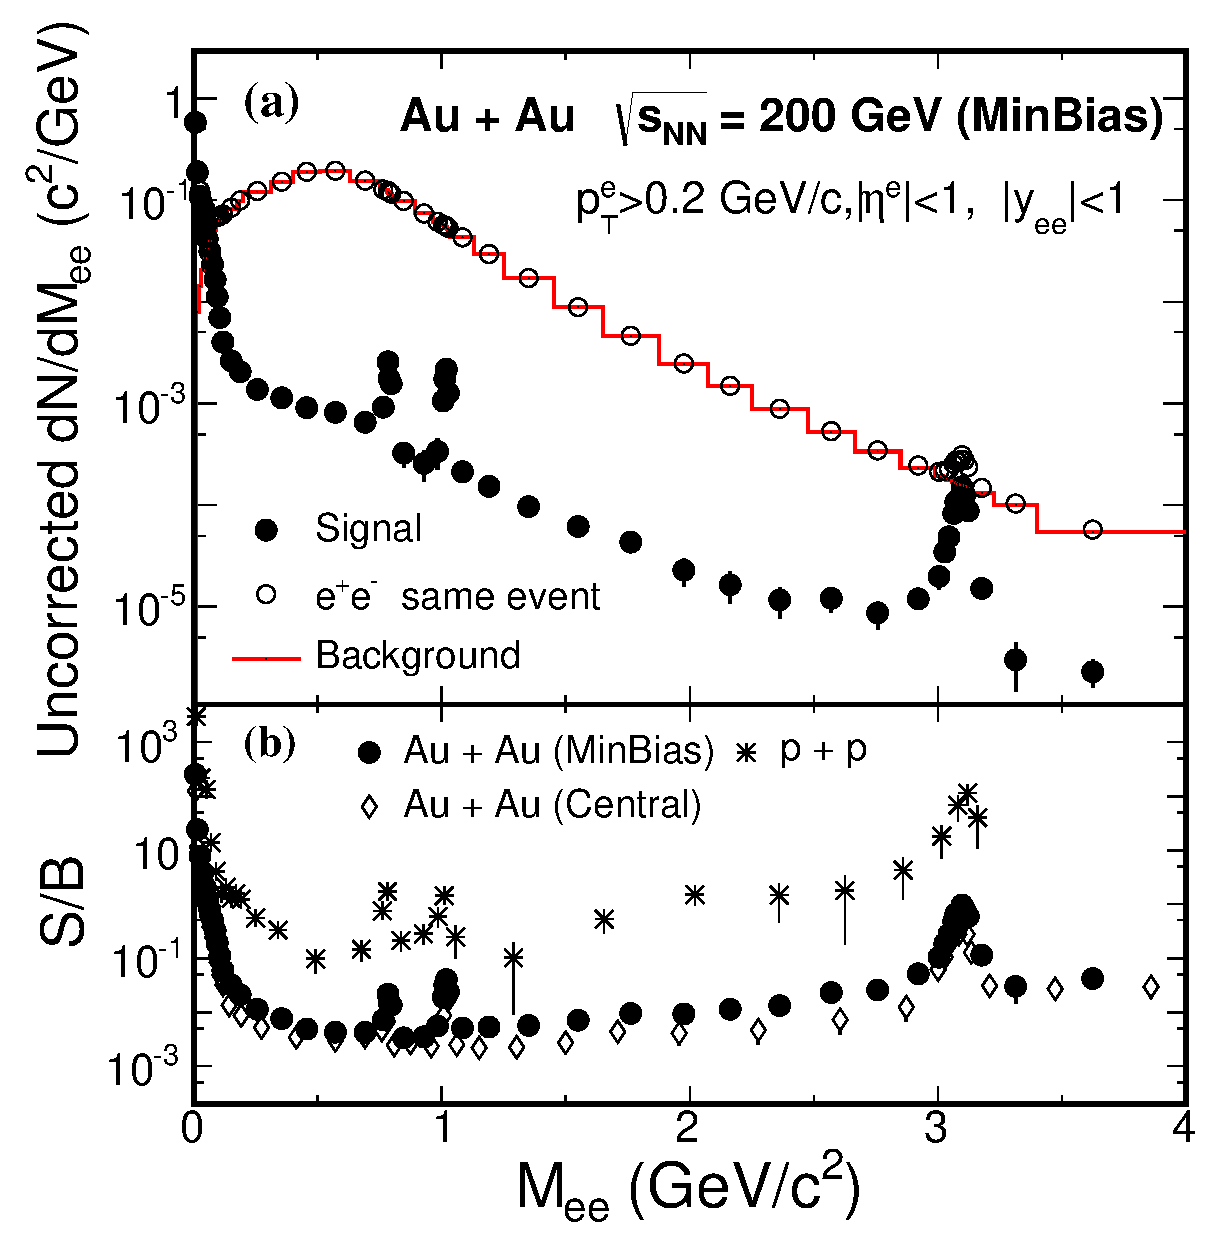
\includegraphics[width=0.45\textwidth]{paper_PRL.eps}
\caption[]{(Color online) (a) Uncorrected distributions of $e^+e^-$ invariant mass (open circles), the reconstructed background (red histogram) and the signal (solid dots) pairs in 200 GeV Au+Au minimum bias collisions. (b) The ratio of signal to background in $p$+$p$~\cite{STARpp} and Au+Au collisions at \sNN = 200 GeV.}
\label{bg1}
\end{figure}



%\begin{figure}[ht]
%\centering
%\includegraphics[width=0.45\textwidth]{sb_PRL.eps}
%\caption[]{Signal to background ratios in dielectron spectra from $p$+$p$~\cite{STARpp} and Au+Au collisions at \sNN = 200 GeV.}
%\label{bg1}
%\end{figure}


%The signal-to-background ratios from $p$+$p$~\cite{STARpp}, Au+Au minimum bias and Au+Au central collisions at \sNN = 200 GeV are shown in Fig.~\ref{bg1}.

% efficiency estimation
The raw signal was corrected for the detector tracking efficiency.
The single electron tracking efficiency was determined using the embedding technique in which Monte Carlo (MC) simulated electrons, propagated through the STAR detector in GEANT~\cite{geant:321} to produce raw signals, are embedded into real data prior to processing with the offline reconstruction software.
The TOF matching and particle identification efficiencies were evaluated based on measured distributions from the real data~\cite{Efficiency}. The dielectron pair efficiency was obtained by convoluting with single electron efficiency and its kinematic dependence. Finally, we corrected for an additional inefficiency at very low-mass due to the photon conversion pair cut.

% systematic uncertainties
The systematic uncertainty in our final mass spectrum is estimated from the following sources: a$)$ uncertainty on the normalization factor for mixed-event background subtraction, 0.06\%, resulting in up to a maximum of 15\% uncertainty at 1\,GeV/$c^2$; b$)$ uncertainty on the residual correlated background resulting in 10\% uncertainty in the mass region of 1-3\,GeV/$c^2$ ; c$)$ uncertainty on the correction factor of the acceptance difference between like-sign and unlike-sign pairs resulting in 5-8\% uncertainty at 0.3-1\,GeV/$c^2$; d$)$ uncertainty due to the hadron contamination in the electron samples resulting in 8\% uncertainty between 1-3\,GeV/$c^2$ and e$)$ uncertainty on the detector efficiency correction, 13\%. The systematic uncertainty in the raw dielectron spectrum is evaluated as the sum of components a$)$-d$)$ applied at each pair mass region. The final systematic uncertainty is calculated as the quadratic sum of the raw spectrum uncertainty and the pair detection efficiency uncertainty e$)$.

% hadron cocktail
In order to disentangle the various sources contributing to the dielectron signal, a hadronic cocktail simulation, performed previously for $p$+$p$ collisions~\cite{STARpp}, was generated for Au+Au collisions at \sNN = 200\,GeV. The simulation included dielectron contributions from decays or Dalitz decays of $\pi^{0}$, $\eta$, $\eta^{\prime}$, $\omega$, $\phi$, $J/\psi$, $c\bar{c}$, $b\bar{b}$ and Drell-Yan (DY) production.
Tsallis blast-wave parametrizations~\cite{TBW} based on RHIC measurements of light hadron spectra ($\pi^{\pm}$, $K^{\pm}$, $\phi$, $p$, $\bar{p}$, high-$p_{\rm T}$ $\eta$)~\cite{DataPion,DataEta,DataPhi,DataJpsi} were used as the inputs to our cocktail simulations.
The same parameters were also applied to mesons which have not yet been measured ($\omega$, $\eta$ at low-$p_{\rm T}$, and $\eta^{\prime}$). The dielectron yields from correlated charm or bottom decays and DY production are based on PYTHIA model~\cite{pythia} calculations in which parameters have been tuned to published STAR measurements~\cite{DataCharm}.
%The input charm pair production cross section is 0.80$\pm$0.36 mb in $p$+$p$ collisions~\cite{DataCharm} and the $e^+e^-$ pairs from correlated charm decays in PYTHIA were scaled by the number-of-binary-collisions ($N_{\rm bin}$) to obtain the correlated charm contribution in the Au+Au collisions.
The input charm pair production cross section is $d\sigma/dy|_{y=0}$ = 171 $\pm$ 26 $\mu$b per nucleon-nucleon collision~\cite{DataCharm} and the $e^+e^-$ pairs from correlated charm decays in PYTHIA were scaled by the number-of-binary-collisions ($N_{\rm bin}$) to obtain the contribution in the Au+Au collisions.
The systematic uncertainty on the cocktail is dominated by the experimental uncertainties on the measured particle yields and spectra. In particular, the large uncertainty in the cocktail in the mass region of 0.15-1\,GeV/$c^2$ is mainly attributed to the unmeasured low-$p_{\rm T}$ $\eta$ mesons and the input charm cross section.


In Fig.~\ref{invMass} (a), a comparison is shown between the hadronic cocktail simulations and the efficiency corrected dielectron yield in 200\ GeV minimum bias Au+Au collisions, in the STAR acceptance range of $p_{\rm T}^e>$0.2 GeV/$c$, $|\eta^e|<$1 and $|y_{ee}|<$1. The hadronic cocktail simulations exclude contributions from the $\rho$ meson to avoid double counting when compared to models. The ratios of our measured data to the cocktail are shown in panel (b) of Fig.~\ref{invMass}. Panel (c) in Fig.~\ref{invMass} shows an expanded view of the excess mass region with the cocktail subtracted.
An enhancement of 1.77$\pm$0.11(stat.)$\pm$0.24(sys.)$\pm$0.33(cocktail) is observed when compared to the hadronic cocktail without the $\rho$ contribution in the mass region of 0.30-0.76\,GeV/$c^2$. This enhancement factor, determined within the STAR acceptance, is significantly lower than what has been reported by PHENIX ~\cite{PHENIX}.
We have compared the STAR and PHENIX cocktail simulations and applied PHENIX azimuthal acceptance. We found that neither differences in the acceptance nor the cocktail simulations can explain the difference in the enhancement factor measured by the two experiments.


\begin{figure}[h]
\centering
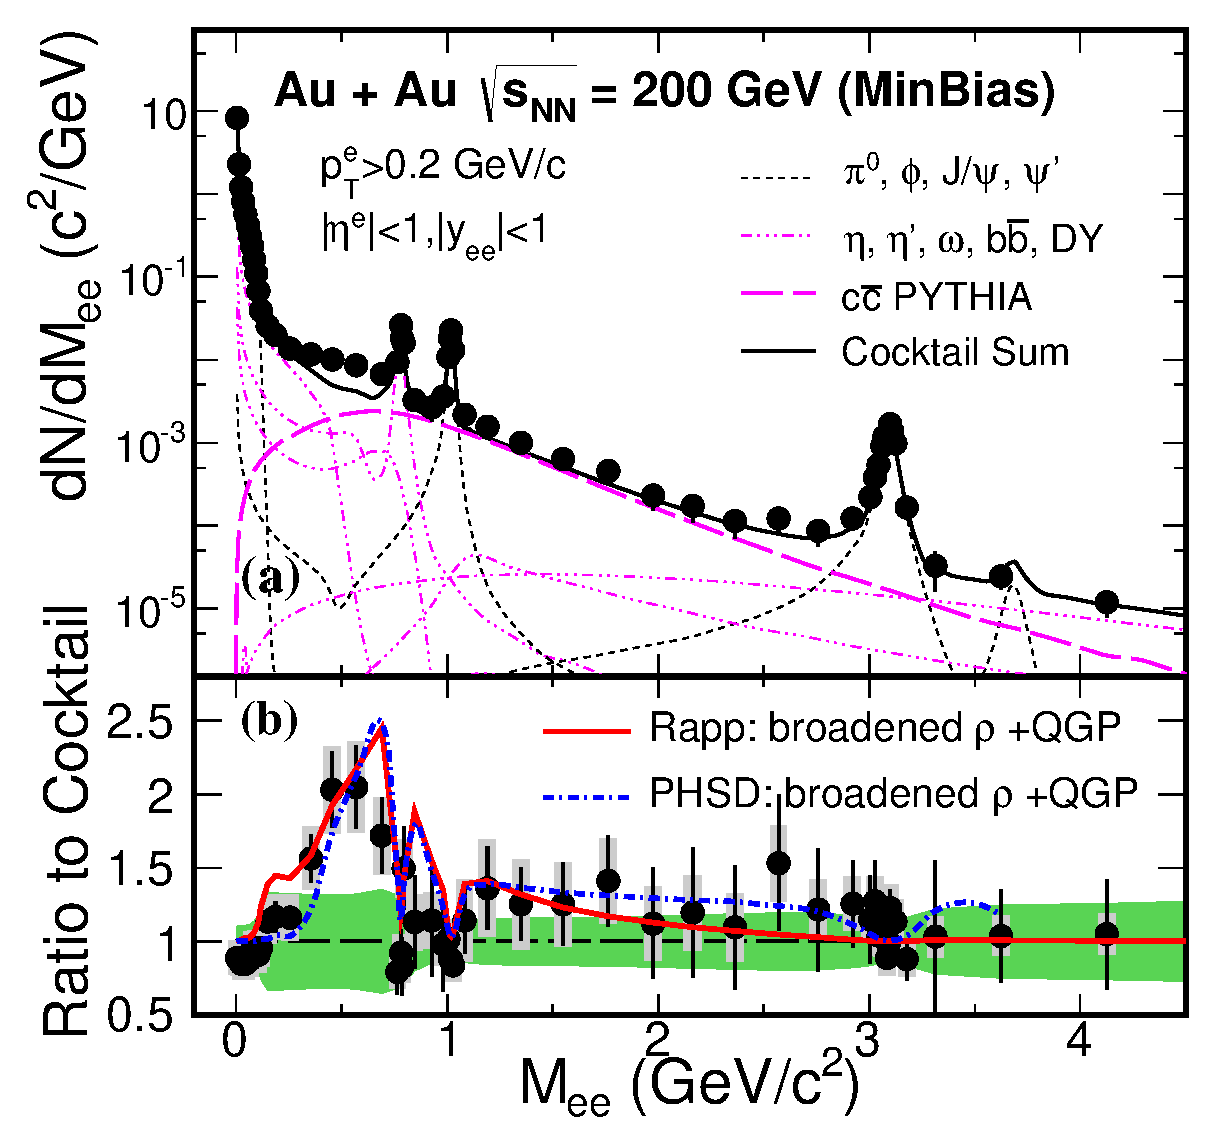
\includegraphics[width=0.45\textwidth]{corrYieldmb_PRL.eps}
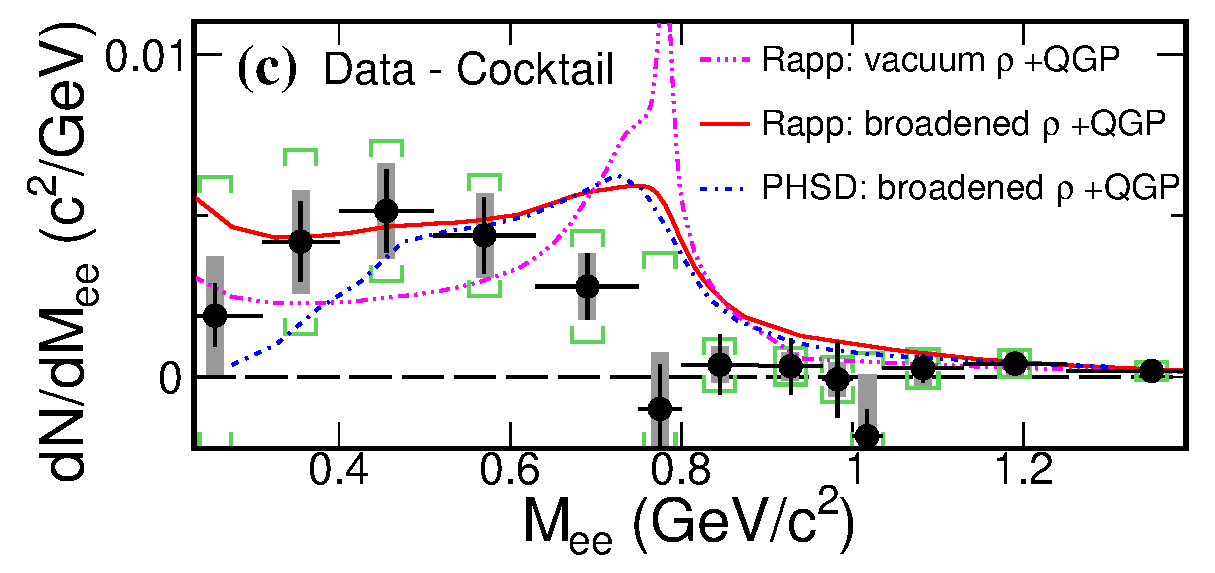
\includegraphics[width=0.45\textwidth]{200mb_excess.eps}
\caption{(Color online) (a) $e^+e^-$ invariant mass spectrum from \sNN = 200 GeV Au+Au minimum bias (0-80\%) collisions compared to a hadronic cocktail simulation.
The vertical bars on data points depict the statistical uncertainties, while the systematic uncertainties are shown as grey boxes (smaller than the marker).
(b) Ratios to cocktail for data and model calculations~\cite{RappPriv,PHSDEE}. Green bands
depict systematic uncertainties on the cocktail.
(c) Mass spectrum of the excess (data minus cocktail) in the low-mass region compared to model calculations. Green brackets depict the total systematic uncertainties including those from cocktails. Systematic errors are highly correlated across all data points.
}
\label{invMass}
\end{figure}

Also included in Fig.~\ref{invMass} (b) and (c) are two theoretical model calculations within the STAR acceptance: Model I by Rapp {\it et al.} is an effective many-body calculation~\cite{RappThermalEE,Rapp4SPS,RappPriv};
Model II by Linnyk {\it et al.} is a microscopic transport model - Parton-Hadron String Dynamics (PHSD)~\cite{PHSD,PHSDEE,PHSD4SPS}. Both models have successfully described the dimuon enhancement observed by NA60 with a broadened $\rho$ spectral function due to in-medium hadronic interactions. The models, however, failed to reproduce the dielectron enhancement reported by PHENIX~\cite{PHENIX,PHSDEE}. Compared to our data in the mass region below 1\,GeV/$c^2$, both models describe the observed dielectron excess reasonably well within uncertainties.
%{\color{red}{\sout{Most $\rho$ mesons produced at chemical freeze-out are still coupled to the hadronic medium and thus are considered as medium contributions in model calculations.}}}
Other theoretical model calculations can also reproduce the dielectron excess at low-mass in our measurement~\cite{HJXu,Vujanovic}.
Our measurements disfavor a pure vacuum $\rho$ spectrum for the excess dielectrons ($\chi^{2}$/NDF= 26/8, where NDF is the number of degrees of freedom, in 0.3-1\,GeV/$c^{2}$).

\begin{figure}[h]
\centering
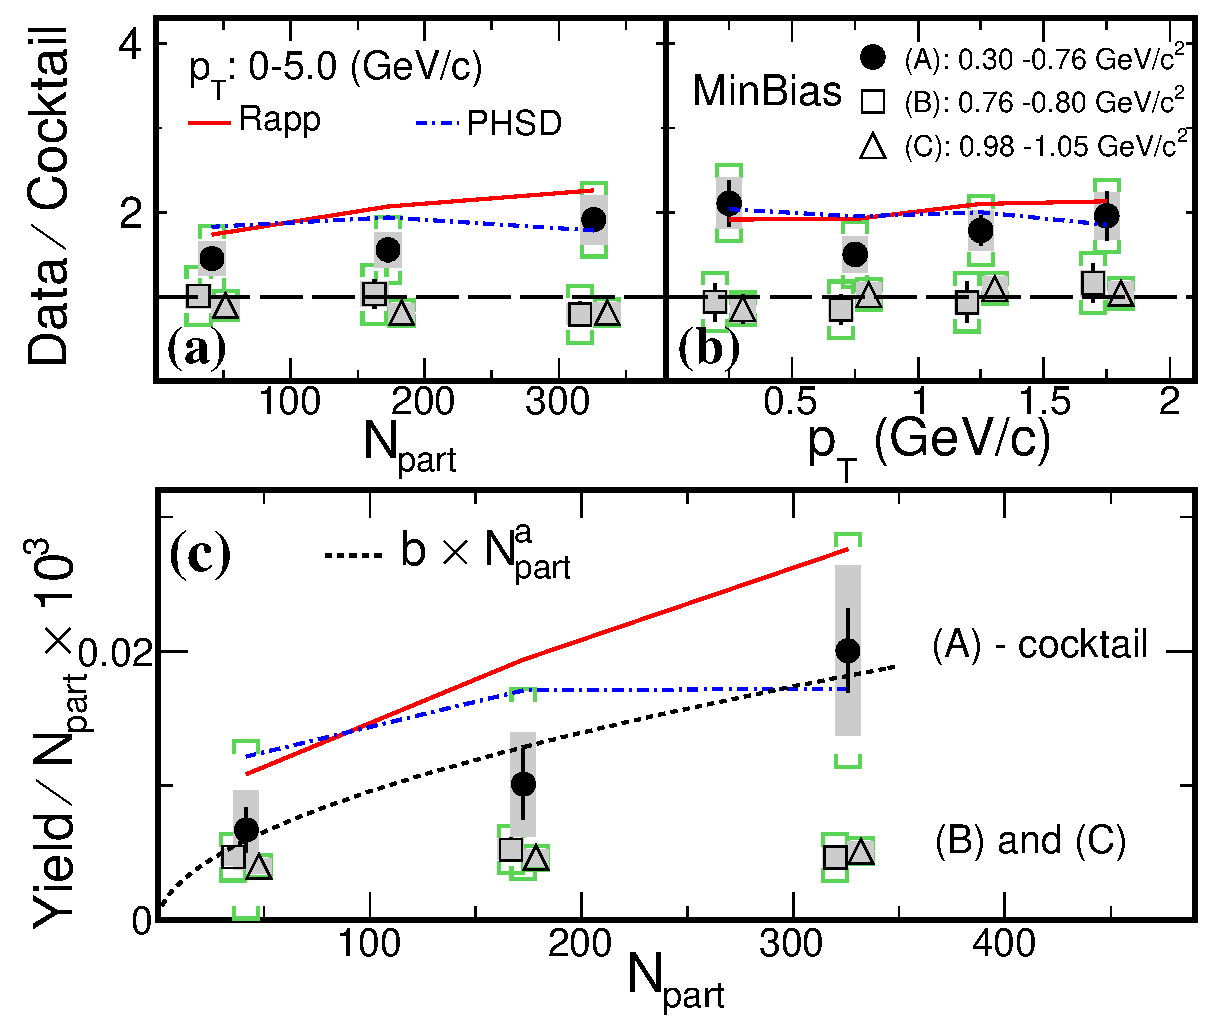
\includegraphics[width=0.45\textwidth] {omega_rho_new.eps}
\caption[]{(Color online) Integrated dielectron yields in the mass regions of 0.30-0.76\,($\rho$-like), 0.76-0.80\,($\omega$-like) and 0.98-1.05\,($\phi$-like) \GeVcsq compared to hadronic cocktails within the STAR acceptance as a function of centrality (a) and dielectron \pT (b). Panel (c) shows the yields scaled by $N_{\rm part}$ for the $\rho$-like region with cocktail subtracted, the $\omega$-like and $\phi$-like regions without subtraction as a function of $N_{\rm part}$. Systematic uncertainties from data are shown as grey boxes, and green brackets depict the total systematic uncertainties including those from cocktails. For clarity, the $\omega/\phi$-like data points are slightly displaced horizontally.}
\label{enhanceCent}
\end{figure}


We integrated the dielectron yields in three mass regions: 0.30-0.76\,($\rho$-like),
0.76-0.80\,($\omega$-like) and 0.98-1.05\,($\phi$-like)\,GeV/$c^2$, and present the centrality and \pT dependence of the ratios of data to cocktail within the STAR acceptance in Fig.~\ref{enhanceCent} (a) and (b).
The cocktail calculation can reproduce the dielectron yields in the $\omega$-like and the $\phi$-like regions.
The ratios to cocktail in the $\rho$-like region show a weak dependence on the number of participating nucleons ($N_{\rm part}$) and $p_{\rm T}$. Both models show excesses comparable to the data in the centrality and $p_{\rm T}$ regions investigated.
Panel (c) shows the integrated yields scaled by $N_{\rm part}$ for the $\rho$-like with cocktail subtracted, the $\omega/\phi$-like without subtraction as a function of $N_{\rm part}$. The $\omega/\phi$-like yields show a $N_{\rm part}$ scaling. The dashed curve depicts a power-law fit ($\propto N_{\rm part}^a$) to the $N_{\rm part}$ scaled $\rho$-like dielectron excess with cocktail subtracted, and the fit result shows $a=0.54\pm0.18$ (stat.+uncorrelated sys.), indicating dielectrons in the $\rho$-like region are sensitive to the QCD medium dynamics, as expected from $\rho$ medium modifications in theoretical calculations~\cite{RappPriv,RhoOmega}.

\begin{figure}[h]
\centering
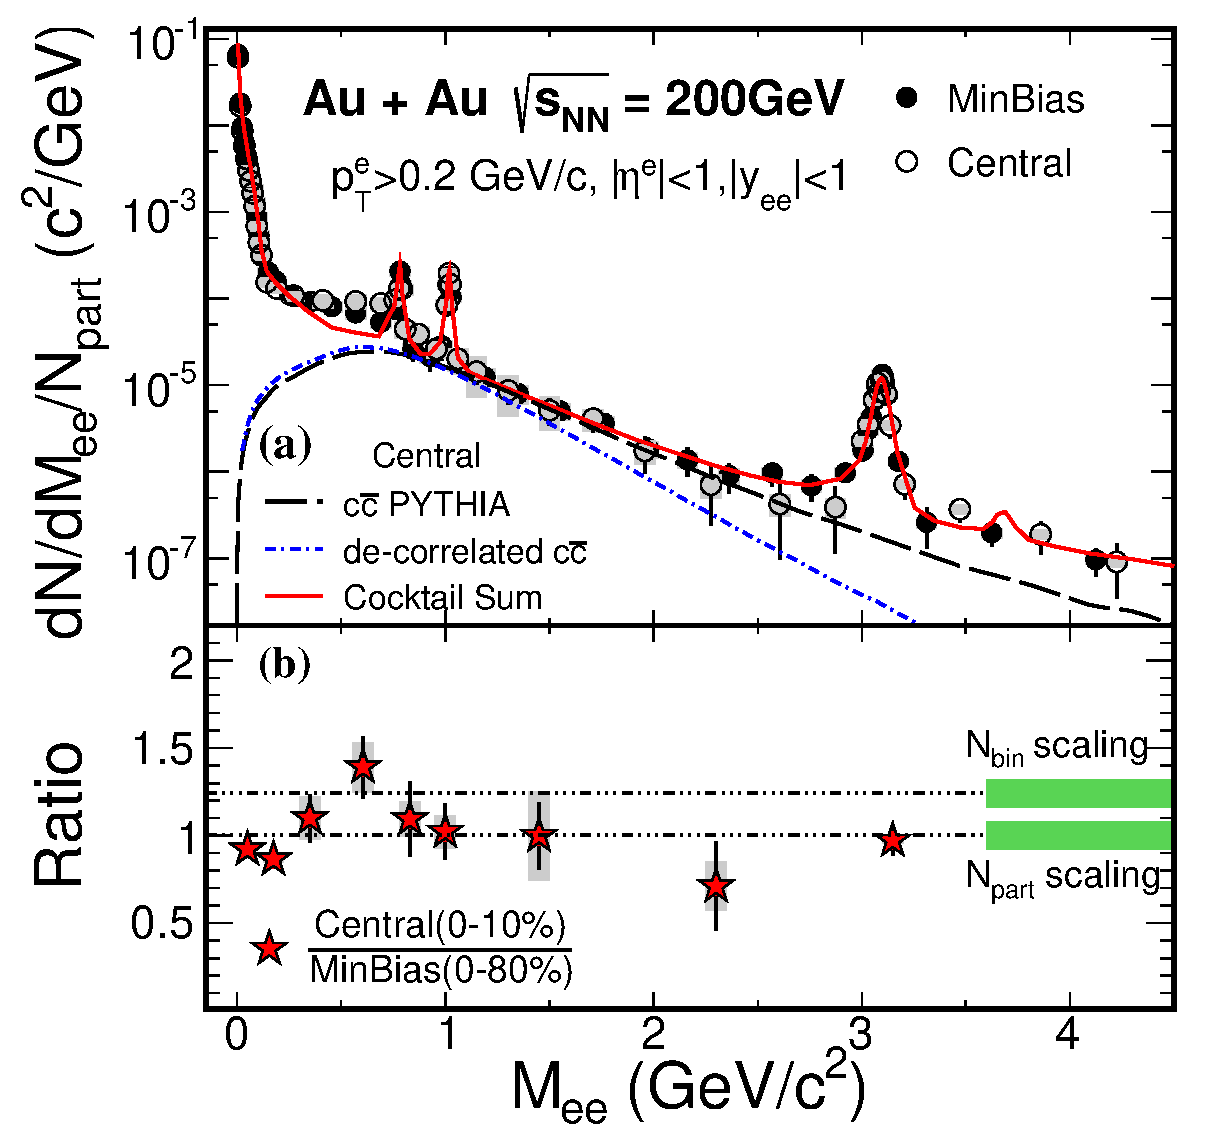
\includegraphics[width=0.45\textwidth] {ee200Rcp.eps}
\caption[]{(Color Online) (a)Dielectron mass spectra scaled with $N_\mathrm{part}$ from minimum bias (0-80\%) and central (0-10\%) collisions. The solid line represents the hadronic cocktail for central collisions. (b) The ratio of $N_\mathrm{part}$ scaled dielectron yields between the central and minimum bias collisions. The grey boxes show the systematic uncertainties on the data.}
\label{dielectronRcp}
\end{figure}

Figure~\ref{dielectronRcp} shows a comparison of the invariant mass spectra between 0-80\% minimum bias and 0-10\% most central Au+Au collisions. Both spectra were scaled by $N_\mathrm{part}$ in panel (a), and the ratios of the two scaled spectra are presented in panel (b).
Horizontal bands on the right side depict the $N_\mathrm{part}$ and $N_\mathrm{bin}$ scaling.
We note that:
(i) The dielectron production starts with the $N_{\rm part}$ scaling in the $\pi^{0}$ and $\eta$ dominant region and then rises towards the $N_{\rm bin}$ scaling at $\sim$0.7\ GeV/$c^2$.
This can be explained by the hadronic medium $\rho$ contribution, which is expected to increase faster than $N_\mathrm{part}$~\cite{RappPriv,RhoOmega}, and the contribution from correlated charm which, if not modified, should follow the $N_{\rm bin}$ dependence. Possible charm de-correlation has negligible impact in this mass region.
(ii) In the mass region of 1-3\ GeV/$c^2$, the ratio between the central and minimum bias spectra shows a moderate deviation from the $N_{\rm bin}$ scaling (1.8$\sigma$ deviation for the data point at 1.8-2.8 GeV/$c^2$).
We have used two extreme scenarios to model the charm decay dielectron pairs: The dashed line in Fig.~\ref{dielectronRcp} (a) depicts the PYTHIA calculation with charm correlations preserved; the dot-dashed line assumes a fully randomized azimuthal correlation between charmed hadron pairs and the \pT suppression factor on the single electron spectrum from RHIC measurements is also included~\cite{NPERaa}.
The difference in the mass region 1-3 GeV/$c^2$, if confirmed with better precision, would constrain the magnitude of the de-correlating effect on charm pairs while traversing the QCD medium and/or possible other dielectron sources (e.g., QGP thermal radiation) in this mass region from central Au+Au collisions.

In summary, we present STAR measurements of dielectron production in Au+Au collisions at \sNN = 200 GeV.
The dielectron yields in the $\omega$ and $\phi$ mass regions are well described by the hadronic cocktail model while yields at higher mass, 1-3\,GeV/$c^2$, can be understood as mostly from decay leptons of charm pairs. In the 0.30-0.76\,GeV/$c^2$ region, however, there exists a clear excess over the hadronic cocktail that cannot be explained by a pure vacuum $\rho$. This enhancement is significantly lower than what has been reported by PHENIX.  Compared to the yields in the $\omega$ and $\phi$ regions, the excess yields in the $\rho$ region exhibit stronger growth with more central collisions.
Theoretical model calculations that include a broadened $\rho$ spectral function from interactions with the hadronic medium can describe the STAR measured dielectron excess at the low-mass region.


%--=======================================================
%\section{acknowledgement}
We thank the RHIC Operations Group and RCF at BNL, the NERSC Center at LBNL, the KISTI Center in Korea,
and the Open Science Grid consortium for providing resources and support. This work was supported in part
by the Offices of NP and HEP within the U.S.DOE Office of Science, the U.S. NSF, CNRS/IN2P3, FAPESP CNPq of
Brazil,the Ministry of Education and Science of the Russian Federation, the NNSFC, the MoST of China (973 Program
No. 2014CB845400), CAS, the MoE of China, the Korean Research Foundation, GA and MSMT of the Czech
Republic, FIAS of Germany, DAE, DST, and CSIR of India, the National Science Centre of Poland, National
Research Foundation (Grant No. NRF-2012004024), the Ministry of Science,Education and Sports of the Republic of
Croatia, and RosAtom of Russia.



%\end{linenumbers}


%--=======================================================
\begin{thebibliography}{999}
% ---

\bibitem{STARwhitepaper} J. Adams {\it et al.} [STAR Collaboration], \Journal{\NPA}{757}{102}{2005};
K. Adcox {\it et al.} [PHENIX Collaboration], \Journal{\NPA}{757}{184}{2005}; B.B. Back {\it et al.} [PHOBOS Collaboration], \Journal{\NPA}{757}{28}{2005}; I. Arsene {\it et al.} [BRAHMS Collaboration], \Journal{\NPA}{757}{1}{2005}.

\bibitem{Shuryak} E. Shuryak, \Journal{\PR}{61}{71}{1980}.

\bibitem{RappThermalEE} R. Rapp, \Journal{\PRC}{63}{054907}{2001}.

%\bibitem{DengDileptonFlow} J. Deng, Q. Wang, N. Xu and P. Zhuang, \Journal{\PLB}{701}{581}{2011}.

%\bibitem{ChatterjeeDileptonV2} R. Chatterjee, D.K. Srivastava, U. Heinz and C. Gale, \Journal{\PRC}{75}{054909}{2007}.

%\bibitem{ShuryakDileptonPol} E. Shuryak, arXiv: 1203.1012.

\bibitem{RappWambach} R. Rapp and J. Wambach, \Journal{\ANP}{25}{1}{2000}.

\bibitem{BrownRho} G.E. Brown and M. Rho, \Journal{\PR}{269}{333}{1996}.

\bibitem{RappWambach2} R. Rapp and J. Wambach, \Journal{\EPJA}{6}{415}{1999}.

\bibitem{DLS} R.J. Porter {\it et al.} [DLS Collaboration], \Journal{\PRL}{79}{1229}{1997}.

\bibitem{HADES} G. Adamova {\it et al.} [HADES Collaboration], \Journal{\PRL}{98}{052302}{2007}; \Journal{\PRC}{84}{014902}{2011}.

\bibitem{HELIOS3} A.L.S Angelis {\it et al.} [HELIOS/3 Collaboration], \Journal{\EPJ}{13}{433}{2000}.

\bibitem{CERES} G. Agakichiev {\it et al.} [CERES Collaboration], \Journal{\PRL}{91}{042301}{2003}; \Journal{\EPJ}{41}{475}{2005}.

\bibitem{NA60} R. Arnaldi {\it et al.} [NA60 Collaboration], \Journal{\PRL}{96}{162302}{2006}; \Journal{\PRL}{100}{022302}{2008}; \Journal{\EPJ}{59}{607}{2009}.

\bibitem{PHENIX} A. Adare {\it et al.} [PHENIX Collaboration], \Journal{\PRC}{81}{034911}{2010}.

\bibitem{Rapp4SPS} H. van Hees and R. Rapp, \Journal{\PRL}{97}{102301}{2006}; H. van Hees and R. Rapp, \Journal{\NPA}{806}{339}{2008}.

\bibitem{Renk4SPS} J. Ruppert, C. Gale, T. Renk, P. Lichard and J. Kapusta, \Journal{\PRL}{100}{162301}{2008}; T. Renk and J. Ruppert, \Journal{\PRC}{77}{024907}{2008}.

\bibitem{Dusling4SPS} K. Dusling, D. Teaney and I. Zahed, \Journal{\PRC}{75}{024908}{2007}.

\bibitem{PHSD4SPS} O. Linnyk, E. L. Bratkovskaya, V. Ozvenchuk, W. Cassing, and C. M. Ko, \Journal{\PRC}{84}{054917}{2011}.

\bibitem{PiKPSpectra} B.I. Abelev {\it et al.} [STAR Collaboration], \Journal{\PRC}{79}{034909}{2009}.

% --============================= STAR technical papers on NIMA
%\bibitem{starnim} Special Issue on RHIC and Its Detectors, edited by M.~Harrison, T.~Ludlam, and S.~Ozaki, \Journal{\NIMA}{499}{No. 2-3}{2003}.

% TPC
\bibitem{tpcnim} M. Anderson, {\it et al.}, \Journal{\NIMA}{499}{659}{2003}.

% TOF proposal
%\bibitem{tofproposal} STAR TOF proposal, \url{http://drupal.star.bnl.gov/STAR/files/future/proposals/tof-5-24-2004.pdf}.
\bibitem{tofnim} W.J. Llope (for the STAR Collaboration), \Journal{\NIMA}{661}{S110}{2012}.

% (p)VPD
%\bibitem{vpdnim} W.J. Llope, {\it et al.}, \Journal{\NIMA}{522}{252}{2004}.

% BEMC
%\bibitem{bemcnim} M. Beddo, {\it et al.}, \Journal{\NIMA}{499}{725}{2003}.

% EEMC
%\bibitem{eemcnim} C.E. Allgower, {\it et al.}, \Journal{\NIMA}{499}{740}{2003}.

% bbc
%\bibitem{bbcnim} J. Kyriluk, \Journal{AIP Conf. Proc.}{675}{424}{2003}.

\bibitem{PIDNIM} M. Shao, O. Barannikova, X. Dong, Y. Fisyak, L. Ruan, P. Sorensen, and Z. Xu, \Journal{\NIMA}{558}{419}{2006}.


% STAR pp dielectron
\bibitem{STARpp} L. Adamczyk {\it et al.} [STAR Collaboration], \Journal{\PRC}{86}{024906}{2012}.

\bibitem{geant:321}GEANT 3.21, CERN program library.
http://wwwasdoc.web.cern.ch/wwwasdoc/geant
\_html3/geantall.html.

\bibitem{Efficiency} J. Zhao, Ph. D. thesis, Shanghai Institute of Applied Physics, 2013. https://drupal.star.bnl.gov/STAR/theses/phd-32.

%\bibitem{STARKstarPhiD} J. Adams {\it et al.}, \Journal{\PLB}{612}{181}{2005}; J. Adams {\it et al.}, \Journal{\PRC}{71}{064902}{2005}; J. Adams {\it et al.}, \Journal{\PRL}{94}{062301}{2005}.

%\bibitem{FlowMethod} A.M. Poskanzer and S.A. Voloshin, \Journal{\PRC}{58}{1671}{1998}; J. Adams {\it et al.}, \Journal{\PRC}{72}{014904}{2005}.


% TBW fit
\bibitem{TBW} Z. Tang, Y. Xu, L. Ruan, G. van Buren, F. Wang, and Z. Xu, \Journal{\PRC}{79}{051901}{2009}; Z.-B. Tang, L. Yi,
L.-J. Ruan, M. Shao, C. Li, H.-F. Chen, B. Mohanty, and
Z.-B. Xu, {Chin. Phys. Lett.} {\bf{30}}, 031201 (2013).

\bibitem{DataPion} J. Adams {\it et al.} [STAR Collaboration], \Journal{\PRL}{92}{112301}{2004}; B.I. Abelev {\it et al.} [STAR Collaboration], \Journal{\PRL}{97}{152301}{2006}; S.S. Alder {\it et al.} [PHENIX Collaboration], \Journal{\PRL}{91}{072301}{2003}; S.S. Alder {\it et al.}, \Journal{\PRC}{69}{034909}{2004}.

%\bibitem{DataPion1} J. Adams {\it et al.} [STAR Collaboration], \Journal{\PRL}{92}{112301}{2004}.

%\bibitem{DataPion2} B.I. Abelev {\it et al.} [STAR Collaboration], \Journal{\PRL}{97}{152301}{2006}.

%\bibitem{DataPion3} S.S. Alder {\it et al.} [PHENIX Collaboration], \Journal{\PRL}{91}{072301}{2003}; S.S. Alder {\it et al.}, \Journal{\PRC}{69}{034909}{2004}.

\bibitem{DataEta} S.S. Adler {\it et al.} [PHENIX Collaboration], \Journal{\PRC}{75}{024909}{2007}.

\bibitem{DataPhi} J. Adams {\it et al.} [STAR Collaboration], \Journal{\PLB}{612}{181}{2005}.

\bibitem{DataJpsi} A. Adare {\it et al.} [PHENIX Collaboration], \Journal{\PRL}{98}{232301}{2007}.

\bibitem{pythia}  T. Sjostrand, P. Edén, C. Friberg, L. Lönnblad, G. Miu, S. Mrenna, and E. Norrbin, {Comput. Phys. Commun.} {\bf{135}}, 238 (2001).

%\bibitem{DataCharm} L. Adamczyk {\it et al.} [STAR Collaboration], \Journal{\PRD}{86}{072013}{2012}.
\bibitem{DataCharm} L. Adamczyk {\it et al.} [STAR Collaboration], arXiv: 1404.6185.
%\bibitem{DataRho} J. Adams {\it et al.} [STAR Collaboration], \Journal{\PRL}{92}{092301}{2004}.

%\bibitem{pdg} C.~Amsler {\it et al.}, \Journal{\PLB}{667}{1}{2008}.

%\bibitem{RappPriv} R. Rapp, private communications.
\bibitem{RappPriv} R. Rapp, PoS CPOD2013, 008 (2013); R. Rapp, private communications.

\bibitem{PHSDEE} O. Linnyk, W. Cassing, J. Manninen, E. L. Bratkovskaya, and C. M. Ko, \Journal{\PRC}{85}{024910}{2012}; O. Linnyk, private communications.

\bibitem{PHSD} W. Cassing and E.L. Bratkovskaya, \Journal{\NPA}{831}{215}{2009}; E.L. Bratkovskaya, W. Cassing, V.P. Konchakovski, and O. Linnyk,  \Journal{\NPA}{856}{162}{2011}.

\bibitem{HJXu} H. J. Xu, H. F. Chen, X. Dong, Q. Wang, and Y. F. Zhang, \Journal{\PRC}{85}{024906}{2012}.

\bibitem{Vujanovic} G. Vujanovic, C. Young, B. Schenke, S. Jeon, R. Rapp, and C. Gale, \Journal{\NPA}{904}{557c}{2013}; G. Gujanovic, C. Young, B. Schenke, R. Rapp, S. Jeon, and C. Gale, \Journal{\PRC}{89}{034904}{2014}.

%\bibitem{HSD} W. Cassing and E.L. Bratkovskaya, \Journal{\PR}{308}{65}{1999}; E.L. Bratkovskaya and W. Cassing,  \Journal{\NPA}{619}{413}{1997}; W. Ehehalt and W. Cassing,  \Journal{\NPA}{602}{449}{1996}.

%\bibitem{Braaten} E. Braaten, R.D. Pisarski and T.C. Yuan, \Journal{\PRL}{64}{2242}{1990}.
\bibitem{RhoOmega} U. Heinz and K.S. Lee, \Journal{\PLB}{259}{162}{1991}.

%\bibitem{Eletsky} V.L. Elestsky {\it et al.}, \Journal{\PRC}{64}{035202}{2001}.

%\bibitem{CSR} R. Rapp, J. Wambach and H. van Hees, arXiv: 0901.3289; R. Rapp, {J. Phys. Conf. Ser.} {\bf{420}}, 012017 (2013).

\bibitem{NPERaa} A. Adare {\it et al.} [PHENIX Collaboration], \Journal{\PRL}{98}{172301}{2007}.


\end{thebibliography}
\end{document}
